\documentclass[twosided]{report}

% Packages %
\usepackage{fancyhdr}
\usepackage{titling}
\usepackage{amsmath}
\usepackage{graphicx}
\usepackage{amssymb}
\usepackage{amsthm}
\usepackage{array}
\usepackage{pifont}
\usepackage{color}
\usepackage{listing}

% Stylings %
\pagestyle{fancy}

% Commands %
\newcommand{\subtitle}[1]{%
  \posttitle{%
    \par\end{center}
    \begin{center}\large#1\end{center}
    \vskip0.5em}%
}

% Footer/Header %
\fancyhead[LE,RO]{\slshape Chapter \thechapter}
\fancyhead[LO,RE]{\slshape \rightmark}
\fancyfoot[C]{\thepage}

\begin{document}

\renewcommand{\arraystretch}{1.5}
\title{OpenNemID 
	\\Bachelor project - Spring 2013}
\subtitle{Verified Secure Open Source Alternative to NemID}
\author{
  Andreas Hallberg Kjeldsen\\
  \texttt{ahal@itu.dk}
  \and
  Morten Chabert Eskesen\\
  \texttt{mche@itu.dk}
}

\date{May 22, 2013}
\maketitle

\begin{abstract}
Your abstract goes here...
\end{abstract}

\tableofcontents 

\chapter{Introduction}

\section{Objectives}
Some explaining text here
\par


\begin{enumerate}
	\item Describe and outline the OpenNemID protocol, including but not limited to registration and login.
	\item Formalize the specification of OpenNemID in F* to the extent possible.
\end{enumerate}

\section{Scope}
This project has had it focus towards specifying a new protocol that could replace NemID. The intent of this project is therefore not to develop a complete system, but to make the specification for a system that could then later be developed based on the specification.

\section{Background}
We're extending the work done by Jacob Højgaard in his Masters Thesis 'Securing Single Sign-On Systems With Executable Models'. Jacobs research has focused on the current implementation of NemID and therefore describes, outlines and models the current system used in Denmark as of May 2013.

\chapter{Static analysis}
This stuff is hard :(


%%%%%%%%%% CHAPTER %%%%%%%%%%
\chapter{Remodelling the protocol}

\section{Communication Model}
The communication model displays a graphical overview of how data should be communicated between the involved parties.
\newpage
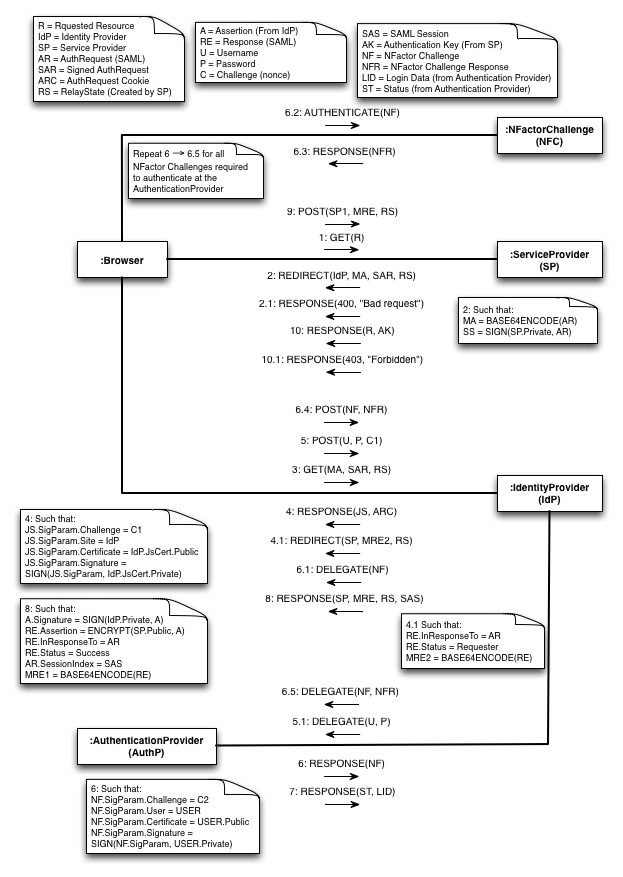
\includegraphics[]{images/Communication.png}

\end{document}